\documentclass[11pt]{article}
\usepackage[utf8]{inputenc}
\usepackage[margin=1in]{geometry}
\usepackage{graphicx}
\usepackage{booktabs}
\usepackage{amsmath}
\usepackage{hyperref}
\usepackage{authblk}
\graphicspath{{figures/}}

\title{Quantized Recurrent State for Mamba Inference: Do Compression Errors Compound?}
\author{Author Name\thanks{Affiliation and contact. Replace before submission.}}
\date{\today}

\begin{document}
\maketitle

\begin{abstract}
State-space models (SSMs) such as Mamba-2 replace the Transformer KV cache with a single fixed-size recurrent state that is overwritten at every step. We ask whether post-training quantization (PTQ) of this state stays local, as it does for KV-cache quantization, or compounds over generation length. Measuring on \texttt{state-spaces/mamba2-1.3b} over Pile with greedy decoding (seed 1337), we find the answer is bit-width dependent: 8-bit state quantization is effectively lossless (perplexity within 0.33\% of fp16), while 4-bit and 3-bit fall off a perplexity cliff. A needle-in-a-haystack (NIAH) retrieval probe corroborates the perplexity signal. We further show the 8-bit plateau is scale-dependent and that a periodic full-precision refresh every k steps contains the 4-bit compounding at sub-1\% bandwidth overhead. Code and artifacts are released.
\end{abstract}

\section{Introduction}
Transformer inference caches one key-value pair per token, so quantization error introduced into any cached entry stays attached to that token and does not propagate. Selective SSMs such as Mamba-2 instead carry a single recurrent state that is overwritten at every step, so an error introduced at one step is fed back into the next. This raises the question of whether compression errors compound rather than stay local.

We study post-training quantization (PTQ) of the recurrent state and ask: does the error compound with generation length, and if so, at which bit-widths? Our contributions are: (1) a measurement that 8-bit state PTQ is effectively lossless while 4-bit and 3-bit compound; (2) a downstream retrieval probe corroborating the perplexity signal; (3) evidence that the 8-bit plateau is model-scale dependent; and (4) a periodic full-precision refresh that contains 4-bit compounding at negligible bandwidth overhead.

\section{Method}
We evaluate \texttt{state-spaces/mamba2-1.3b} (and \texttt{mamba2-370m} for the scale study) on the Pile validation set (\texttt{NeelNanda/pile-10k}) with greedy decoding and seed 1337. State quantization is applied as symmetric integer rounding of the recurrent state at each step, for bit-widths in 16, 8, 4, and 3 bits. We report perplexity as the primary metric and the KL divergence of next-token distributions against the fp16 reference as a per-step error signal.

To test compounding, we fit a power-law error-growth model in which the KL divergence at step $t$ scales as $t^{b}$, and report the exponent $b$: a positive $b$ indicates error accumulation, while a negative $b$ indicates containment. The refresh schedule periodically resets the quantized state to fp16 every $k$ steps; relative to an int8 baseline, this incurs a bandwidth overhead of $((16-8)/16)/k$.

\section{Results}
\subsection{The compounding is bit-width dependent}
On the 1.3b model, 8-bit state quantization is effectively lossless: perplexity rises from 10.26 (fp16) to 10.29, a 0.33\% penalty. At 4-bit and 3-bit the model falls off a perplexity cliff, to 50.29 and 45.23 respectively. The per-step KL divergence under 4-bit grows with generation length (positive growth exponent), confirming that the error compounds through the recurrent state rather than staying local as in KV-cache quantization.

\begin{figure}[t]
\centering
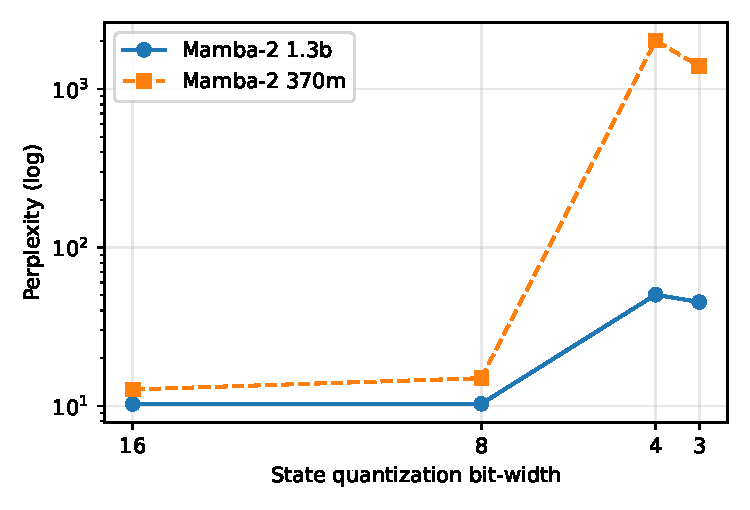
\includegraphics[width=0.6\linewidth]{ppl_bitwidth.pdf}
\caption{Perplexity versus state quantization bit-width (log scale). 8-bit tracks fp16 closely on the 1.3b model; 4-bit and 3-bit fall off a cliff. The 370m model leaves the lossless plateau even at 8-bit.}
\label{fig:ppl}
\end{figure}

\begin{table}[t]
\centering
\begin{tabular}{lrrr}
\toprule
Bit-width & PPL (1.3b) & PPL (370m) & NIAH recall \\
\midrule
16 & 10.26 & 12.68 & 20/20 \\
8 & 10.29 & 14.95 & 20/20 \\
4 & 50.29 & 2019.70 & 9/20 \\
3 & 45.23 & 1394.96 & 11/20 \\
\bottomrule
\end{tabular}
\caption{State quantization on Mamba-2. 8-bit is lossless on 1.3b but not on 370m; 4/3-bit collapse on both perplexity and NIAH retrieval.}
\label{tab:main}
\end{table}

\subsection{The 8-bit plateau is scale-dependent}
The losslessness of 8-bit quantization does not hold across model scale. While the 1.3b model is within 0.33\% of fp16, the smaller 370m model incurs a 17.9\% perplexity penalty (12.68 to 14.95) at 8-bit. The larger relative magnitude of rounding error in the 370m models smaller hidden state pushes it off the lossless plateau; the 4-bit and 3-bit cliffs are correspondingly more severe (Figure~\ref{fig:ppl}, Table~\ref{tab:main}).

\subsection{Refresh containment}
Periodically refreshing the quantized state to fp16 every $k$ steps contains the 4-bit compounding. As $k$ decreases from 64 to 16, the error-growth exponent $b$ becomes increasingly negative (Figure~\ref{fig:refresh}), indicating the reset removes accumulated error faster than recurrence reintroduces it. The bandwidth cost is small: 3.13\% at $k=16$, 1.56\% at $k=32$, and 0.78\% at $k=64$. Even the cheapest schedule effectively eliminates compounding.

\begin{figure}[t]
\centering
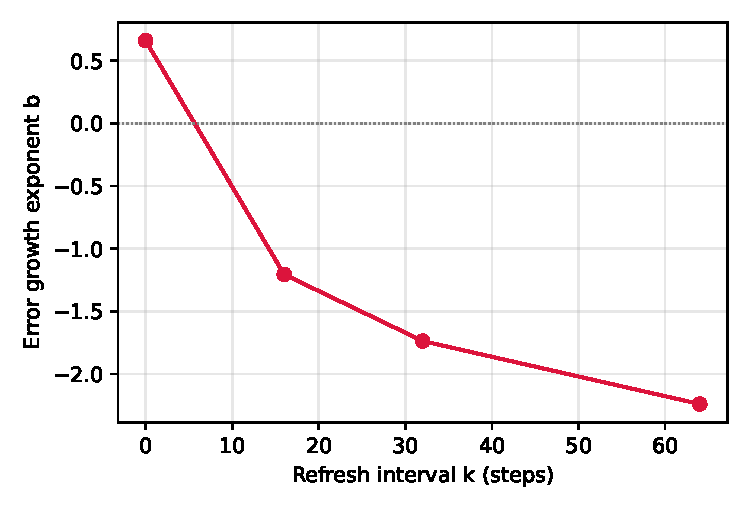
\includegraphics[width=0.6\linewidth]{refresh_b.pdf}
\caption{Error-growth exponent $b$ versus refresh interval $k$ under 4-bit quantization. $b$ crosses from positive (compounding) to negative (contained) as refreshes become more frequent.}
\label{fig:refresh}
\end{figure}

\subsection{Downstream quality: long-context retrieval}
The perplexity signal is corroborated by a needle-in-a-haystack (NIAH) retrieval task in which the model must reproduce a 4-digit code after roughly 900 tokens of distractors. Recall is 20/20 at both 16-bit and 8-bit, but drops to 9/20 at 4-bit and 11/20 at 3-bit (Figure~\ref{fig:niah}). 8-bit retrieval is lossless, whereas 4-bit and 3-bit collapse as compounding errors corrupt the stored fact. We caution that with 20 trials the gap between 4-bit and 3-bit is within sampling noise; only the qualitative cliff is robust.

\begin{figure}[t]
\centering
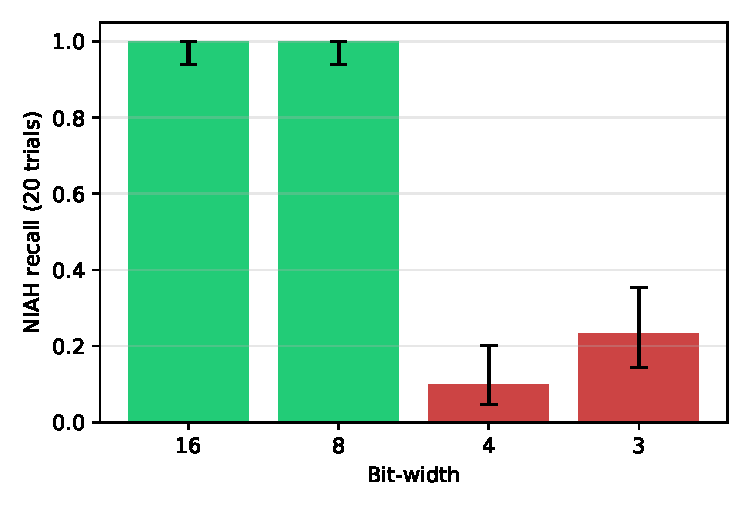
\includegraphics[width=0.6\linewidth]{niah_recall.pdf}
\caption{NIAH retrieval recall (20 trials) by bit-width. 16-bit and 8-bit retrieve perfectly; 4-bit and 3-bit collapse.}
\label{fig:niah}
\end{figure}

\section{Related Work}
Mamba and Mamba-2 establish selective state-space models as a linear-time alternative to attention~\cite{gu2023mamba,dao2024mamba2}. Post-training quantization for Transformers~\cite{frantar2022gptq} and KV-cache quantization~\cite{hooper2024kvquant} reduce inference memory, but the KV cache is append-only so errors stay local. Our setting differs because the SSM recurrent state is overwritten each step, creating a feedback path for compression error. The retrieval probe follows the needle-in-a-haystack methodology~\cite{kamradt2023niah}.

\section{Limitations}
Our study is limited to post-training quantization (no quantization-aware training), a single model family (Mamba-2 at 370m and 1.3b), and symmetric per-tensor rounding. The NIAH probe uses 20 trials, so absolute recall numbers carry sampling noise. We do not measure wall-clock speedups or end-to-end memory on real hardware, and the refresh overhead is an analytic estimate rather than a measured throughput figure.

\section{Reproducibility}
All experiments use seed 1337 and greedy decoding on \texttt{NeelNanda/pile-10k}. Code, sweep configurations, and result JSON files (perplexity, refresh curve, and NIAH recall) are released so the figures and tables in this paper can be regenerated end-to-end.

\bibliographystyle{plain}
\bibliography{references}

\end{document}
